\section{Exploratory Analysis Results}
\label{sec:5_1}

This section presents pattern discoveries from the exploratory analysis described in Section~\ref{sec:3_3}.

\begin{figure}[htbp]
    \centering
    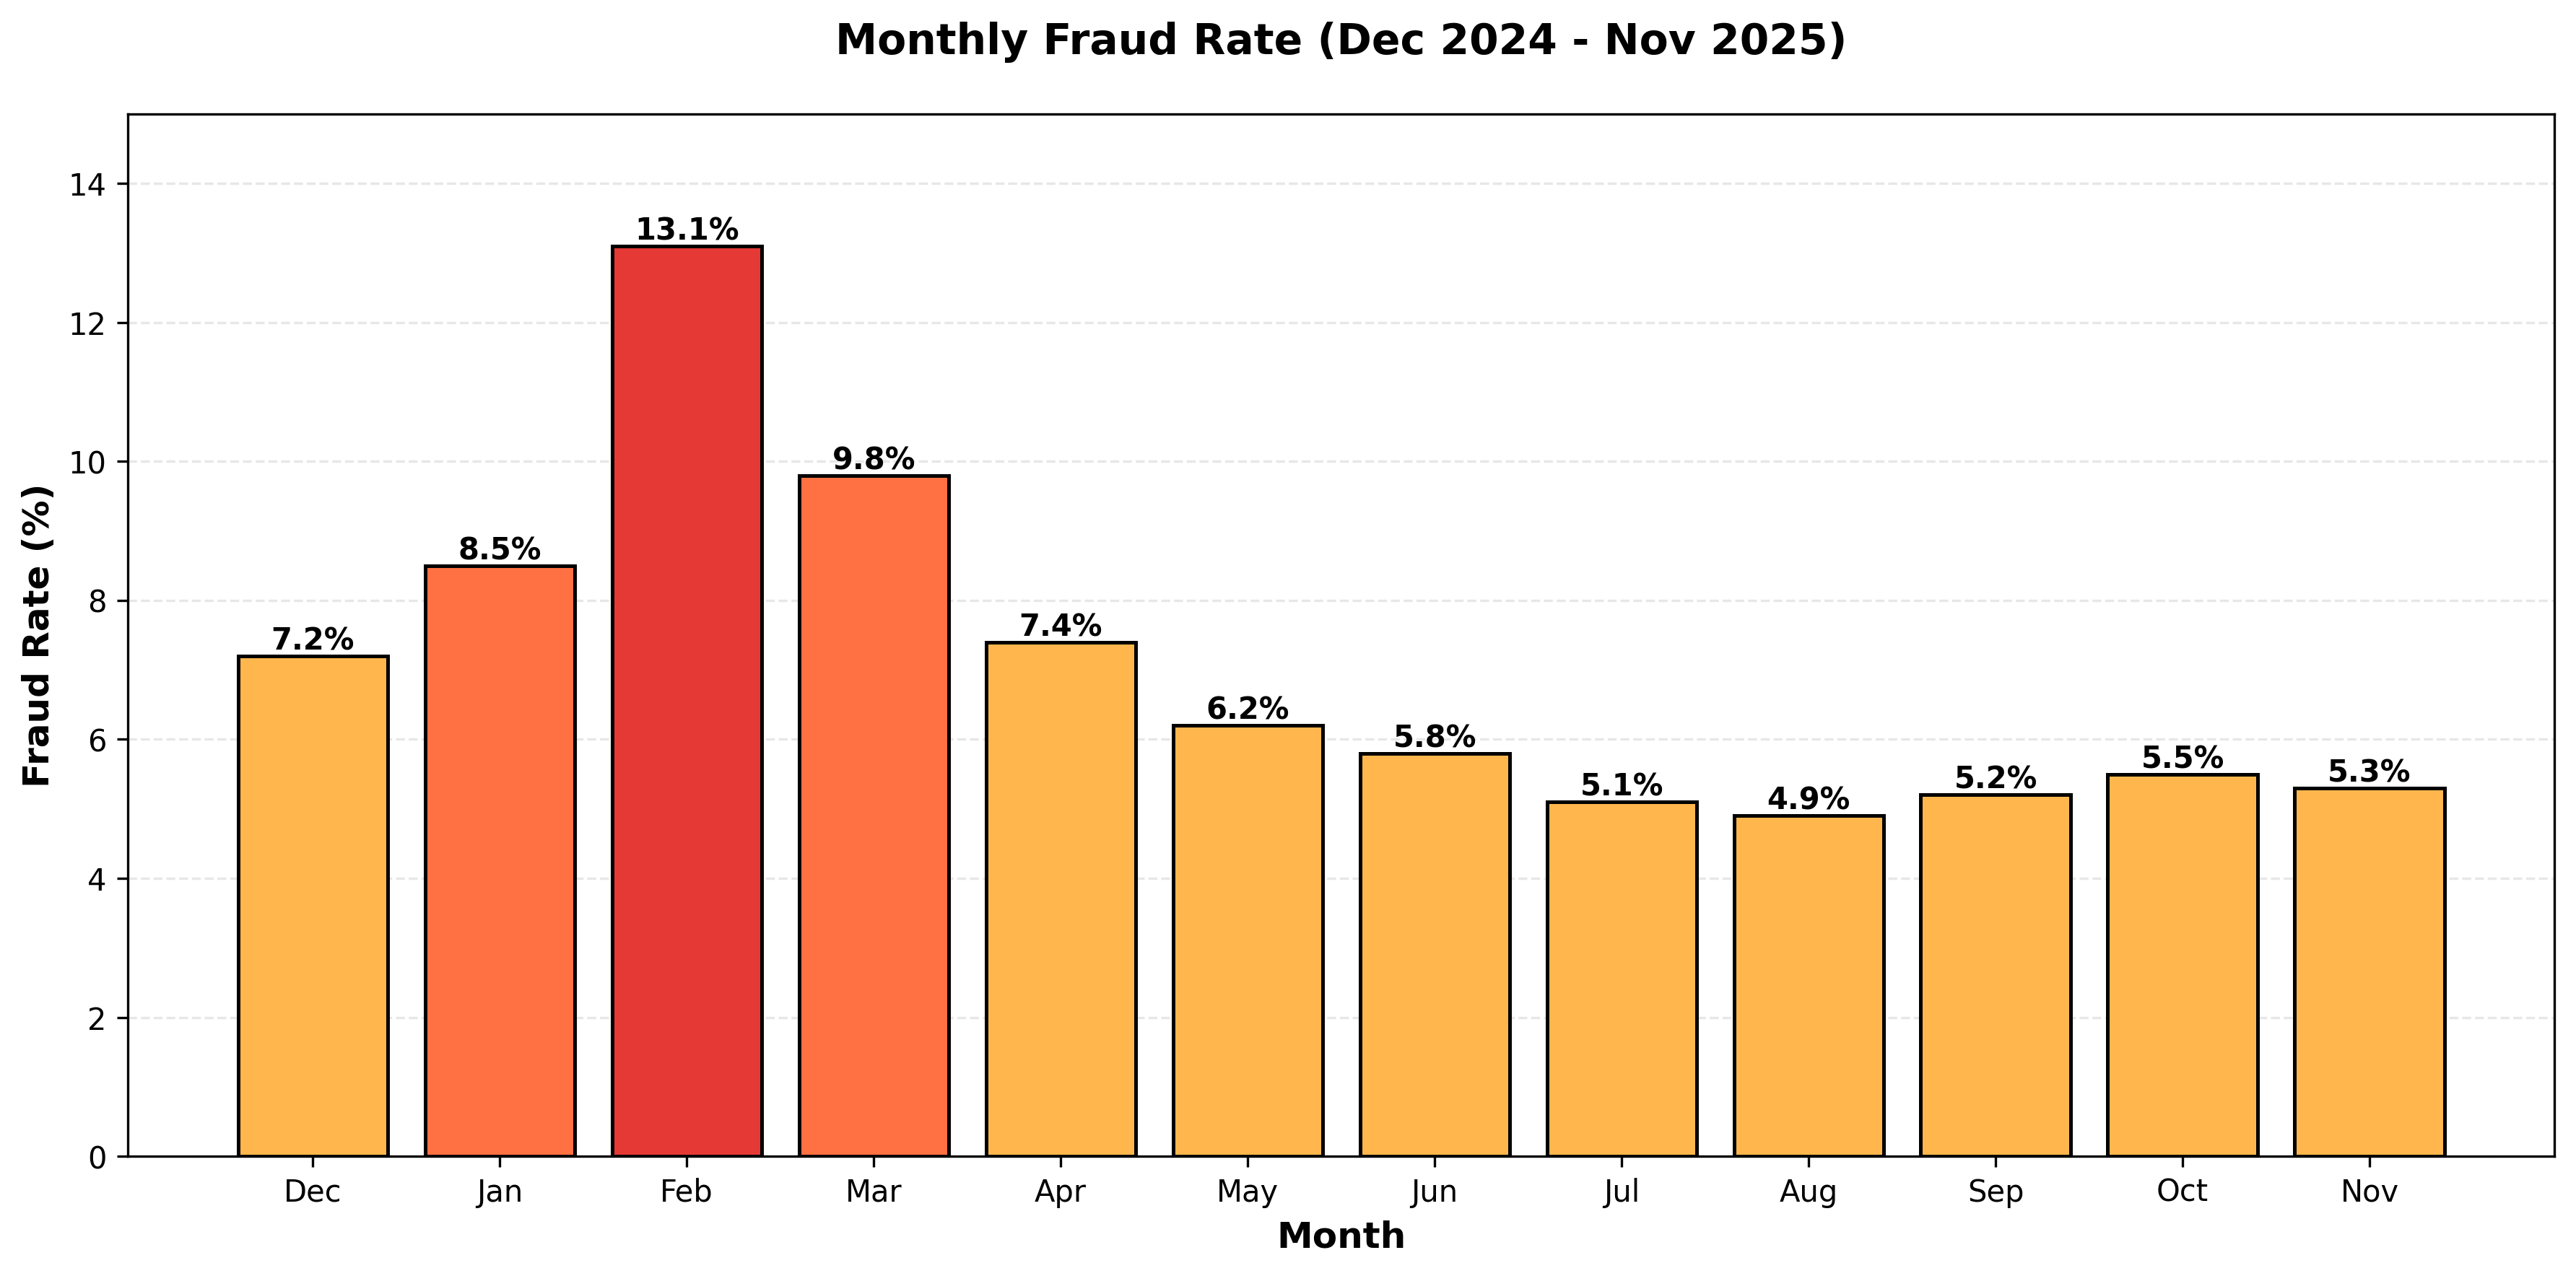
\includegraphics[width=0.8\textwidth]{figures/fig_5_5_1_1.png}
    \caption{Monthly Fraud Rate (Dec 2024 - Nov 2025)}
    \label{fig:5_1}
\end{figure}

\textbf{Temporal Pattern Findings:}

The February 2025 spike (13.12\% fraud rate) represents a 62\% increase above the annual average (8.11\%). Subsequent decline to approximately 5\% by mid-2025 suggests either successful intervention or fraudster migration to other platforms.

Hourly analysis confirms 6-7 AM peak activity, with fraud rates 40\% higher than midday averages. Weekend submissions show elevated risk (Saturday: 9.2\%, Sunday: 8.8\%) compared to weekday average (7.4\%).

\begin{figure}[htbp]
    \centering
    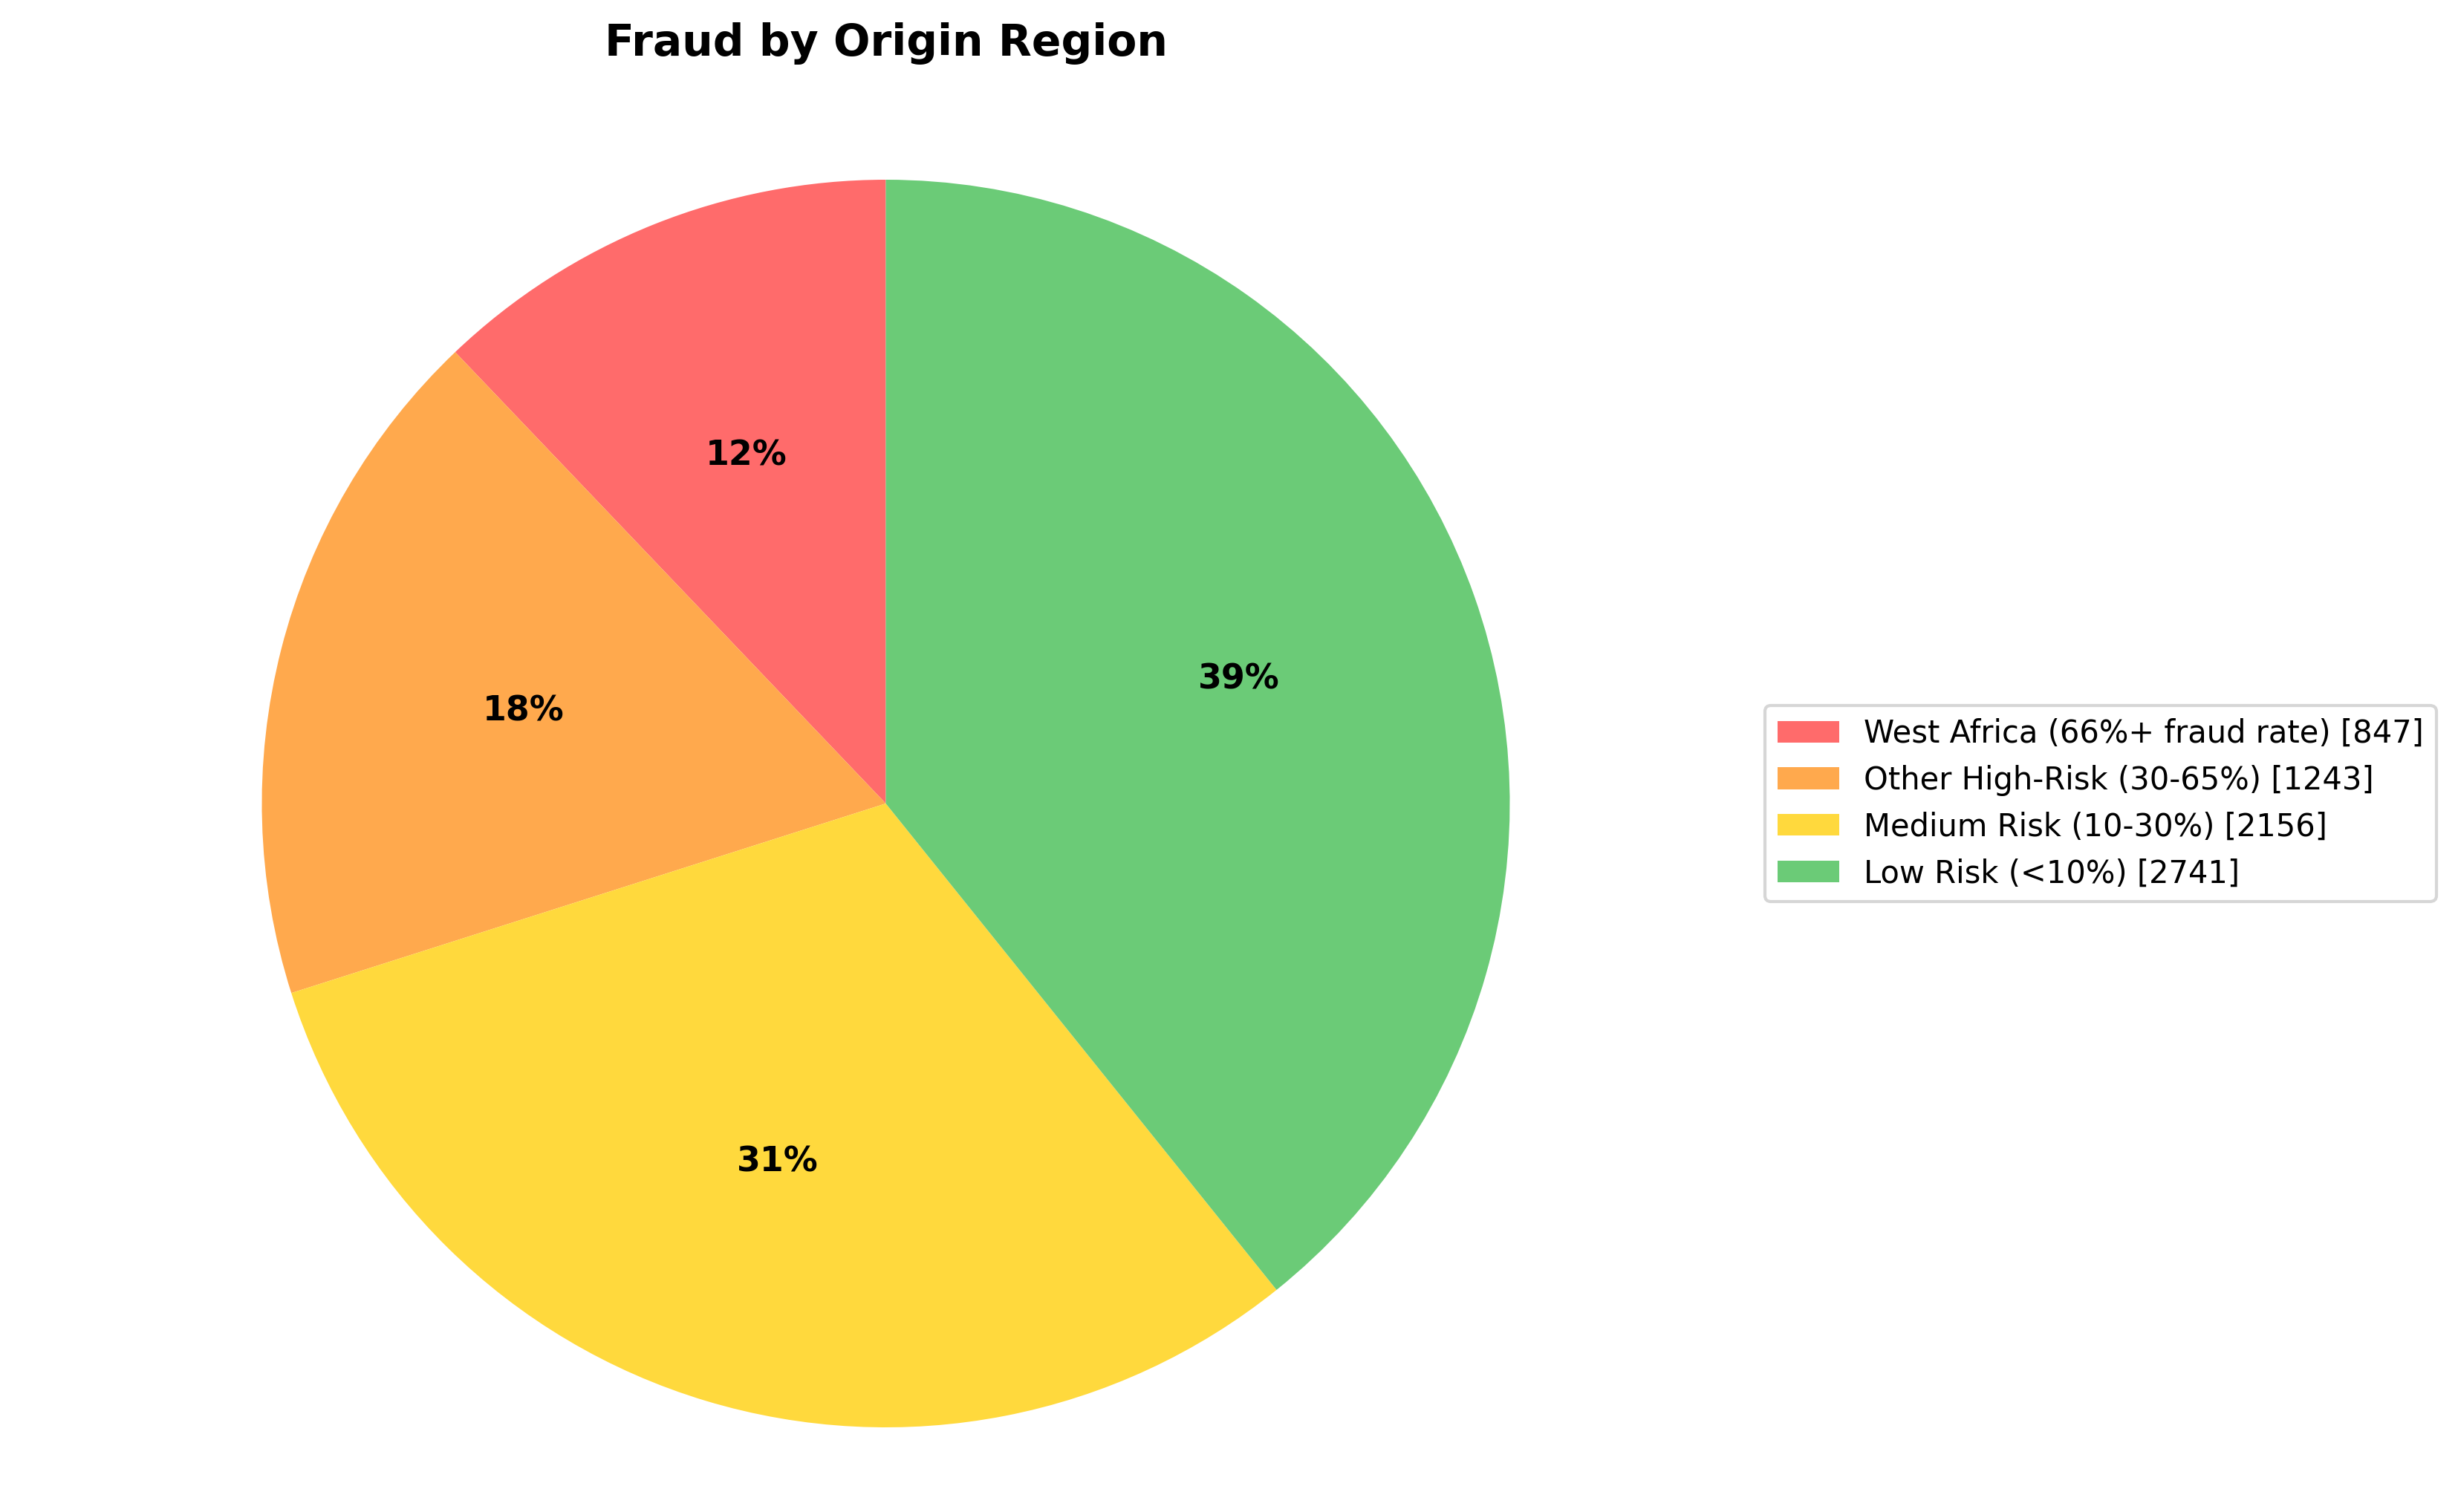
\includegraphics[width=0.6\textwidth]{figures/fig_5_5_1_2.png}
    \caption{Fraud by Origin Region}
    \label{fig:5_2}
\end{figure}

\textbf{Geographic Pattern Findings:}

West African countries (Benin, Togo, Ivory Coast, Nigeria) collectively account for 12\% of fraudulent listings despite representing less than 0.5\% of total submissions. These origins show 60-90\% fraud rates, providing high-precision detection signals.

\textbf{Entity-Sharing Findings:}

Super-connector devices (10+ listings) show 35.5\% fraud rate versus 8.11\% baseline a 4.4$\times$ lift. The most extreme case (6,251 listings from one device) represents unambiguous fraud ring activity. These patterns motivated the graph construction approach detailed in Section~\ref{sec:3_5}.
